\documentclass[10pt, titlepage, oneside, a4paper]{article}
\usepackage[T1]{fontenc}
\usepackage[english]{babel}
\usepackage{ifpdf}
\usepackage{amssymb, graphicx, fancyheadings}
\usepackage{rotating}

\addtolength{\textheight}{20mm}
\addtolength{\voffset}{-5mm}
\renewcommand{\sectionmark}[1]{\markleft{#1}}

\def\inst{Computing Science}
\def\typeofdoc{Project Plan}
\def\course{Software Engineering, Spring 2010, 15 hp}
\def\pretitle{Laboration 3}
\def\title{The Greed Game}
\def\namea{Fredrik Dahlberg}
\def\nameb{Marcus Karlsson}
\def\namec{Emil Eriksson}
\def\usernamea{c07fdg}
\def\usernameb{marcusk}
\def\usernamec{c07een}
\def\emaila{\usernamea{}@cs.umu.se}
\def\emailb{\usernameb{}@cs.umu.se}
\def\emailc{\usernamec{}@cs.umu.se}
\def\path{edu/pvt/lab3}
\def\graders{Tor Sterner Johansson}

\def\fullpatha{\raisebox{1pt}{$\scriptstyle \sim$}\usernamea/\path}
\def\fullpathb{\raisebox{1pt}{$\scriptstyle \sim$}\usernameb/\path}
\def\fullpathc{\raisebox{1pt}{$\scriptstyle \sim$}\usernamec/\path}

\begin{document}

	\begin{titlepage}
		\thispagestyle{empty}
		\begin{large}
			\begin{tabular}{@{}p{\textwidth}@{}}
				\textbf{Ume� University \hfill \today} \\
				\textbf{Department of \inst \hfill } \\
				\textbf{\typeofdoc} \\
			\end{tabular}
		\end{large}
		\vspace{10mm}
		\begin{center}
			\LARGE{\pretitle} \\
			\huge{\textbf{\course}}\\
			\vspace{10mm}
			\LARGE{\title} \\
			\vspace{5mm}
			\begin{large}
				\begin{tabular}{ll}
					\textbf{Name} & \namea \\
					\textbf{Email} & \texttt{\emaila} \\
					\textbf{Path} & \texttt{\fullpatha} \\
					\\
					\textbf{Name} & \nameb \\
					\textbf{Email} & \texttt{\emailb} \\
					\textbf{Path} & \texttt{\fullpathb} \\
					\\
					\textbf{Name} & \namec \\
					\textbf{Email} & \texttt{\emailc} \\
					\textbf{Path} & \texttt{\fullpathc} \\
				\end{tabular}
			\end{large}
			\vfill
			\large{\textbf{Grader}}\\
			\mbox{\large{\graders}}
		\end{center}
	\end{titlepage}

	\lfoot{\footnotesize{\usernamea, \usernameb, \usernamec}}
	\rfoot{\footnotesize{\today}}
	\lhead{\sc\footnotesize\title}
	\rhead{\nouppercase{\sc\footnotesize\leftmark}}
	\pagestyle{fancy}
	\renewcommand{\headrulewidth}{0.2pt}
	\renewcommand{\footrulewidth}{0.2pt}

	\pagenumbering{roman}
	\tableofcontents
	
	\newpage

	\pagenumbering{arabic}
	
	\section{Description}
	
	The project aims to implement a dice game called Greed. It is a turn-based game where a player throws a number of dice and has the ability to register scores depending on a set of rules.

	A player has to reach a lower limit called the bust limit. If the first roll in a turn does not reach that limit the player is bust and the turn will be given to the next player. If the player does not go bust it will have the option to either stop and register the collected scores or roll again and try to collect more points. There must always be at least one die that scores in each roll. If no die scores the player goes bust and the score collected in that turn will be lost. When a die has scored it cannot be used again until all dice has scored.

	This project will implement a GUI-based version of the Greed game. Any number of players may enter or leave the game at any time and they should be able to play from different computers.

	Computer controlled players should also be supported. At least the following four types should be implemented.

	\begin{itemize}
	\item \emph{Coward}, will play safe and not take any risks.
	\item \emph{Random}, will play randomly.
	\item \emph{Clever}, will play cleverly and make tactical decisions, i.e. based on the scores of the other players.
	\item \emph{Gambler}, will play to win as fast as possible by taking very high risks.
	\end{itemize}

	\section{Initial design}
	
	\begin{figure}[t]
		\centering
			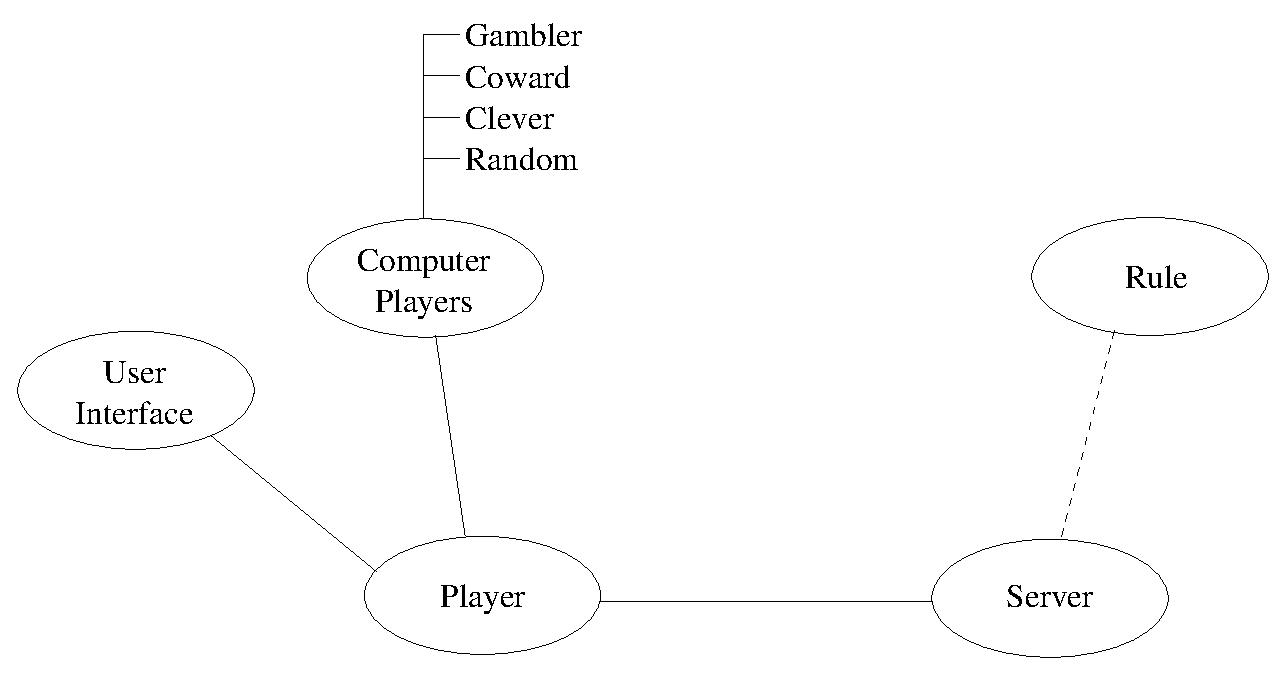
\includegraphics[width=0.8\textwidth]{design.eps}
		\caption{Initial design draft.}
		\label{fig:design}
	\end{figure}
	
	Our initial thoughts on software design is illustrated in figure \ref{fig:design} (\pagename{} \pageref{fig:design}). In order to let players play from different computers the software will be divided into two parts, a client and a server. The server is used by one or many clients. Several players may share the same client simultaneously. In order to make the design more generalized the client-server communication will be utilized even if only one client is used and the server is running on the same computer.

	The server will keep track of all players, their scores and be responsible for rolling the dice. When the turn has come to a player that player will be given the dice throws and then respond with its decision. The server will then send a notification to all clients about the status of the game and let the player continues until the turn is given to another player.

	Since the game exists in several variants it should be fairly easy to add or change rules. A plug-in architecture will be used to dynamically load rules. Adding a rule will therefore not be more difficult than adding a file. Computer controlled player types will also be handled in this way, making it easy to add more of them.
	
	\section{Work breakdown}
	
	\begin{table}[t]
		\vspace{15mm}
		\centering
			\begin{tabular*}{0.8\textwidth}{@{\extracolsep{\fill}} l  c c}
				\multicolumn{1}{c}{\begin{rotate}{45}\textbf{Milestone}\end{rotate}} & \begin{rotate}{45}\textbf{Deadline}\end{rotate} & \begin{rotate}{45}\textbf{Estimated} (hrs)\end{rotate}\\
				\hline
				\hline
				Interfaces \& Blackbox tests
					& 2010-03-03 & 6 \\
				Computer Players 
					& 2010-04-06 & 18 \\
				Rules 
					& 2010-04-07 & 6 \\
				User Interface Designed
					& 2010-04-07 & 10 \\
				Server 
					& 2010-04-09 & 20 \\
				User Interface Implemented
					& 2010-04-13 & 20 \\
				Integration 
					& 2010-04-14 & 6 \\
				\hline
				Project Plan 
					& 2010-03-29 & 20 \\
				Progress Report 
					& 2010-04-08 & 15 \\
				Final Report 
					& 2010-04-15 & 25 \\
					\hline
					\hline
					\textbf{Total estimated time} && 116 \\
					\hline
					\hline
			\end{tabular*}
		\caption{Milestones and time estimations}
		\label{tab:milestones}
	\end{table}
	
		As can be seen in \tablename{} \ref{tab:milestones} (\pagename{} \pageref{tab:milestones}) the work is broken down into several milestones. The "Estimated time"-column represents the time estimated to complete each individual milestone. The milestones will not necessarily be completed one after the other but work will with all certainty be done in parallell on several parts of the project.

		\subsection{Schedule}
		
			In accordance with \tablename{} \ref{tab:milestones} the first week will see the completion of the interfaces and implementation of the computer players.
			
			During the second week the server should be implemented, the user interface designed and the progress report written.
			
			Implementation of the user interface and integration testing will be done during week three as well as the writing of the final report.

	\section{Quality assurance}
		The primary ways that will be used to measure and assure the quality of the system is as follows. 
			LOC - Lines of code the system consists of.
			Test Coverage - Checks how big part of the code that is covered by tests. The goal is to cover everything, 100\%.
			Cyclomatic Complexity - Checks the complexity for every method in each class. The number indicates how complex a method is, so the aim is to have low nubers.
			Coupling - How coupled the different classes are. Reasonably low coupling is to be wanted as it makes it easier to maintain the system.
			LCOM - Lack of cohesion of methods measures how well the modules(classes) are built. A high LCOM means the cohesion is low, and indicates that a class could need to be divided into two or several (sub)classes.
	\section{Tools}

		As Ruby has been chosen as the language for implementation some of the standard tools used in the previous projects aren't available. In the following sections the replacement tools will be described as well as some of the tools used previously.
			
		\subsection{Language}
		
			As mentioned previously Ruby will be used for implementation. Ruby is an interpreted language created by Yukihiro ''matz'' Matsumoto by blending his favorite languages (Perl, Smalltalk, Eiffel, Ada, and Lisp). The result is a language that tries to balance functional programming with imperative programming.
			
			More information on Ruby can be found on http://www.ruby-lang.org/.
		
		\subsection{Unit testing}
		
			For unit testing the module Test::Unit, which is part of the Ruby core will be used.
		
		\subsection{Metrics}
		
			There exist a measurement suite for Ruby called {\tt metric\_fu}. Caliper is a web service which uses this suite to generate statistics.
			
			It is not yet decided whether the web service will be used or the measurement suite will be used as is.

	\section{Project goals}

	The overall goal of the project is to implement the Greed game software that fulfills the specification. The specification will be used to measure how well the software conforms to the requirements that they list. Apart from fulfilling the specification a goal is that the software should be well working.

	\section{Assumptions and risks}

	There are a few risks involved in the project. There is a risk that the project will run out of time, therefore making it a priority to keep tracking of the progress on a day to day basis.

	Another risk is that unfamiliarity to the chosen programming language will cause delays. Two of the team members have previously experienced Ruby and is more or less familiar to it while the third team member has not used it before.

	There are still many unknown factors and this makes it important to keep reevaluating the initial planning during the early stage of the project. As the project progresses it will be more fragile to unknowns and changes to the plan.  For it to be successful thorough planning and preparations for such changes have to be made.

\end{document}
